\documentclass[10pt,a4paper]{article}
\usepackage[T1]{fontenc}
\usepackage[utf8]{inputenc}
\usepackage{mathptmx}
\usepackage{microtype}
\usepackage[margin=2.3cm]{geometry}
\usepackage{booktabs}
\usepackage{graphicx}
\usepackage[font=small,labelfont=bf]{caption}
\usepackage{xcolor}
\usepackage[hidelinks]{hyperref}
\usepackage{url}
\urlstyle{tt}
\usepackage{titlesec}
\titlespacing*{\section}{0pt}{9pt}{3pt}
\titlespacing*{\subsection}{0pt}{6pt}{2pt}
\setlength{\parindent}{1.2em}
\setlength{\parskip}{0pt}
\clubpenalty=10000
\widowpenalty=10000
\raggedbottom
\title{\vspace{-1.2cm}Does LLM-guided patch search speed up the Garmin FIT SDK decoder?\\\large A greedy-chain versus best-of-$N$ study}
\author{Zhou Ziang (A0359536N)\\CS6219 project}
\date{November 2026}
\begin{document}
\maketitle\vspace{-0.6cm}
\begin{abstract}\noindent
We test whether LLM-guided patch search speeds up full-file decode in the Garmin FIT SDK (21.201.0) and whether any gain exceeds repeated independent sampling of the same model. With deepseek-v4.1-flash we compare a \emph{greedy} chain (each call edits the current best patch) with \emph{best-of-N} (each call starts from stock): 40 HTTP requests per run, five seeds per arm, plus compiler-flag (C1) and human-patch (C2) controls. A frozen decision rule (alpha = 0.01, at least a 2\% reduction) was calibrated on synthetic pairs: 0/100 false accepts on the null pair, 99/100 detections at a 4.8\% reduction, 42/100 at 1.965\%. Re-measuring each run's fixed final patch three times, greedy reached a median speedup of 1.169 (range 1.157--1.216) and best-of-N 1.073 (1.067--1.074); greedy was higher in all five seed pairs, used more tokens (median 481k versus 326k) but had the higher speedup per token. \emph{Limits:} best-of-N stays below -O3 (1.090) and near the human patches (1.068, 1.082); only greedy exceeds -O3 -march=native (1.108). The call budgets are unequal (three greedy runs stopped at 38, 34 and 34 of 40 requests at the cluster job limit), and the 34-request comparison, which agrees, was added after the full results were seen. With five seeds, one model, one library and arms that differ in several respects, these exploratory results do not show an advantage of greedy at equal resources and cannot be attributed to selection, feedback or inheritance alone.
\end{abstract}
\section{Problem and method}
\textbf{Question.} Claims that an LLM inside a search loop finds better code than people or compilers \cite{romera2024,novikov2025} usually rest on a few case studies. The course brief asks for the missing control: the same number of model calls without feedback or selection. On one library we ask whether LLM search speeds up the full decode of stock FIT SDK 21.201.0 \cite{garminfit}, and whether it beats best-of-N at the same number of calls. Every candidate is a unified diff of \path{src/}; we report what our modification changed, not a comparison with a vendor product.

\textbf{Search.} One call picks one function (of 5,514 indexed, at most 250 lines each): 90\% of draws are proportional to \emph{perf} samples of a 20 s profile of the stock decode, 10\% are uniform. The model receives the function's text and the stock decode time and returns a replacement body (final \texttt{message.content} only). The patch is built, checked (Section 2.3) and timed. \textbf{Greedy} shows the function as it is under the current best patch and continues from an accepted candidate; a rejected call changes nothing. \textbf{Best-of-N} (control C3) always shows stock and never sees a score, an earlier patch or an error. Both arms use the same model (\texttt{deepseek-v4.1-flash}, always answered as \texttt{deepseek-v4.1-flash-1017}), prompt template, \texttt{max\_tokens} 32768, sampling code and rank rule, and a budget of 40 HTTP requests per run: every request sent counts (truncated replies and 502 errors included), a failure before any request is recorded but not counted, a reply cut at the token limit is never a candidate, and there are no hidden retries.

\textbf{Rank rule and confirmation.} A candidate is measured once; if its ratio r$_1$ is below the current record and the measurement is stable it is measured again, R = max(r$_1$, r$_2$), and the record is replaced only if R is below it. This is an \emph{ordering heuristic} for small gains, not the decision rule of Section 2 and not a significance test. Only each run's final patch is a confirmed result: it is fixed and re-measured three times, independently, under the frozen decision rule. Intermediate steps were never independently confirmed.

\textbf{Chronology and environment.} On 3 November we ran a different model (qwen3-coder-next) with a population search and best-of-N (\path{runs/main/}); on 4 November we changed both model and strategy (greedy). The two experiments differ in two ways; the earlier model runs are archived and not analysed here, except the compiler and human controls (C1, C2), which involve no model. Also kept: a model preflight (21 calls, 249956 tokens; 5/7, 3/7, 0/7 replies truncated at 8192, 16384, 32768 tokens, so \texttt{max\_tokens} = 32768; one reply at 8192 came from another model, \texttt{glm-5.3-flash}, so the returned id is checked), smoke runs, and an invalid first-batch -O3 -march=native control (rerun used). Workload: four generated FIT files, 907,007 bytes, 34,251 messages, 428,714 fields, output checksum \texttt{92bebfd7f8978fc8} (\texttt{bench.err}, identical in all runs). Each formal run used one compute node (xcnc2, xcnc3, xcnc41, xcnd1, xcnd2, xcnd3, xcnd4, xcnd5, xcnd6; 24 logical CPUs, Xeon E5-2620 v3, see Section 4), c++ (Ubuntu 13.3.0-6ubuntu2\textasciitilde{}24.04.1) 13.3.0, SDK flags \texttt{-O2 -std=c++17 -fPIC -fvisibility=hidden} (tools: Release \texttt{-O3 -DNDEBUG}), Google Benchmark 1.9.1, \texttt{--repeat 10 --repetitions 9}, SDK \texttt{--min-time} 0.25 s. Only ratios are compared across node families.

\section{Measurement and calibration}
\subsection{Decision rule}
One measurement runs stock and candidate in the same process (the candidate loaded first in half of the processes), 10 fresh processes $\times$ 9 repetitions. The rule reads each process's \texttt{candidate\_ns} and \texttt{reference\_ns} (\texttt{timings}), takes ratio = median over processes of median(candidate)/median(reference), and applies an exact two-sided sign-flip test to the ten process-level log ratios (2$^{10}$ patterns). \emph{Faster} means mean log ratio below 0, p < 0.01 (alpha) and ratio $\le$ 0.98; \emph{unstable} means a spread of process ratios above 0.25. The unit of analysis is the process-level log ratio; the test assumes the ten processes are independent and, under no difference, symmetric about 0. Repetitions inside a process are not assumed independent (only their median is used). Thresholds were fixed before any calibration data. The null run of \texttt{CanMehHarness init} was clean in all 10 runs (null ratio 0.9992--1.0015, on each run's own node).

\subsection{Phase 0 calibration}
Synthetic pairs differ only in work units, so the true ratio is known by construction. They were measured with \texttt{--repeat 10 --repetitions 9} and each pair's own recorded \texttt{--min-time} (about 0.06 s for the main pairs, larger for sweeps; the SDK uses 0.25 s, so calibration and SDK differ). Main pairs: 100 valid trials (two batches of 50, node xcnc2, Xeon E5-2620 v3); sweep pairs: 20 trials (batch 1 only). Table~\ref{tab:calib} gives the single-measurement outcomes; bias is the median reported ratio minus the true ratio.

\begin{table}[t]
\centering
\small
\setlength{\tabcolsep}{3.5pt}
\begin{tabular}{lrrrrcrr}
\toprule
Pair & Work ref/cand & min-time & True ratio & Trials & Accepted (95\% CI) & Reported & Bias \\
\midrule
null & 20000/20000 & 0.0611 & 1.00000 & 100 & 0 (0.0--3.6\%) & 1.00038 & +0.00038 \\
faster-1\% & 20000/19801 & 0.0609 & 0.99005 & 100 & 1 (0.0--5.4\%) & 0.98973 & -0.00032 \\
faster-2\% & 20000/19607 & 0.0614 & 0.98035 & 100 & 42 (32.2--52.3\%) & 0.98084 & +0.00049 \\
faster-5\% & 20000/19047 & 0.0618 & 0.95235 & 100 & 99 (94.6--100.0\%) & 0.95380 & +0.00145 \\
faster-10\% & 20000/18181 & 0.0610 & 0.90905 & 100 & 100 (96.4--100.0\%) & 0.90926 & +0.00021 \\
slower-10\% & 20000/22000 & 0.0671 & 1.10000 & 100 & 0 (0.0--3.6\%) & 1.10090 & +0.00090 \\
\midrule
sweep-105 & 20000/21000 & 0.0649 & 1.05000 & 20 & 0 (0.0--16.8\%) & 1.05200 & +0.00200 \\
sweep-110 & 20000/22000 & 0.0674 & 1.10000 & 20 & 0 (0.0--16.8\%) & 1.10048 & +0.00048 \\
sweep-200 & 20000/40000 & 0.1218 & 2.00000 & 20 & 0 (0.0--16.8\%) & 2.00759 & +0.00759 \\
sweep-400 & 20000/80000 & 0.2403 & 4.00000 & 20 & 0 (0.0--16.8\%) & 4.02555 & +0.02555 \\
\bottomrule
\end{tabular}
\caption{Phase 0, single-measurement decisions of the frozen rule. min-time in seconds. Reported = median reported ratio; bias = reported $-$ true ratio. CI: 95\% Clopper--Pearson \cite{clopper1934}. Above the rule: main pairs (100 trials); below: sweep pairs (20 trials, batch 1). Source: \path{runs/phase0b-1069564/final/rule_rows.jsonl}.}
\label{tab:calib}
\end{table}
The null pair accepted 0 of 100 (95\% upper bound 3.6\%): alpha = 1\% is the test's threshold, not a measured rate, and 100 null trials cannot show a false-accept rate below 1\%. The weakest tested effect accepted in at least 90\% of trials is the 4.8\% reduction (99/100). The 2\% pair (true reduction 1.965\%, just below the 2\% gate) was accepted 42/100 times, which reflects an effect near the magnitude gate together with measurement fluctuation; noise cannot be excluded. Bias was at most 0.15\% of the true ratio at the main pairs. The sweep pairs (true ratios 1.05--4.00) check that the reported ratio scales with the work count (bias at most 0.026, 0.64\% at 4.0). In the 12-pair self-check \texttt{broken-digest} was refused at stage \texttt{correctness} and \texttt{shared-install-name} at stage \texttt{load}. The calibration is of the \emph{final decision rule}, not of the greedy ranking heuristic, and it scales a whole synthetic workload, whereas a real patch speeds up one part of a decode.

\textbf{Repetition independence.} Lag-1 autocorrelation of each process's 9-value \texttt{candidate\_ns} series (standard error about 0.33 per series), recomputed from raw timings by \path{scripts/autocorr_report.py} (it reproduces the rule's stored values to 1e-14). Median across a measurement's processes, summarised as median [range of those medians] over measurements: calibration main pairs $-$0.10 [$-$0.41, +0.26] (600 measurements); SDK inert patch +0.24 [+0.12, +0.40] (6); SDK search candidates +0.05 [$-$0.31, +0.40] (338); fixed final patches +0.04 [$-$0.18, +0.30] (30). Calibration is slightly negative, SDK slightly positive: SDK repetitions are not known to be independent, which the rule does not assume.

\subsection{Correctness checks and the inert patch}
Before timing, \texttt{CanMehBench} requires that (i) both libraries fold the decoded values to the same 64-bit digest, unchanged on a second decode; (ii) a \emph{profile digest} agrees, which calls \texttt{Profile::GetMesg} for every message number 0--65535 and \texttt{GetFieldIndex}/\texttt{GetField} for every field number 0--255 (nine probes for absent messages); and (iii) neither library works on a second thread (processor over wall time at most 1.15), which rejects candidates that start threads but does not test concurrent callers. These checks do not prove semantic equivalence on all inputs or platforms. An inert patch spliced into the SDK and evaluated by hand gave a median speedup of 1.0001 (5 measurements, 0/5 accepted), so speedups near 1.00 carry no information.

\section{Results}
\textbf{Two analyses, not one experiment.} \emph{Full runs} are what was executed. All best-of-N runs sent 40 requests; greedy seeds 1 and 2 sent 40 (seed 1 stopped at its 9,600 s deadline after 39 requests and was completed by a resume job on another node, tokens included); greedy seeds 3, 4 and 5 stopped at their search deadline (9,300 s, set to fit the three-hour job limit) after 38, 34 and 34 requests. The \emph{34-request analysis} is \textbf{post hoc}: for each run, the best patch under the then-current ranking within its first 34 HTTP requests. The value 34 is the shortest run's request count, taken after the full results were known; it was not chosen by performance but was not specified in advance. Six of the ten 34-request patches equal the final patch and reuse its re-measurement; four differ and were re-measured three times each. The 20 analysis entries (10 final, 10 at 34 requests) therefore rest on 14 distinct patches, and all 20 passed the frozen rule in 3 of 3 re-measurements.

\begin{table}[t]
\centering
\small
\setlength{\tabcolsep}{3.5pt}
\begin{tabular}{llllrrrrrr}
\toprule
Seed & Arm & Node & Req. & Wall (h) & Tok. (k) & Trunc. & Speedup & Metric A & Metric B \\
\midrule
1 & greedy & xcnc3$\rightarrow$xcnd7 & 40 & 2.80 & 621 & 5 & 1.157 & 2.50 & 2.53 \\
 & best-of-N & xcnc41 & 40 & 1.60 & 272 & 0 & 1.073 & 2.69 & 2.68 \\
2 & greedy & xcnc41 & 40 & 2.69 & 597 & 2 & 1.216 & 3.60 & 3.61 \\
 & best-of-N & xcnc2 & 40 & 1.74 & 299 & 1 & 1.069 & 2.28 & 2.30 \\
3 & greedy & xcnd1 & 38 & 2.76 & 351 & 0 & 1.169 & 4.79 & 4.81 \\
 & best-of-N & xcnd4 & 40 & 2.40 & 370 & 1 & 1.074 & 2.00 & 2.00 \\
4 & greedy & xcnd2 & 34 & 2.82 & 452 & 2 & 1.191 & 4.21 & 4.22 \\
 & best-of-N & xcnd5 & 40 & 2.30 & 326 & 0 & 1.073 & 2.22 & 2.23 \\
5 & greedy & xcnd3 & 34 & 2.75 & 481 & 2 & 1.165 & 3.46 & 3.43 \\
 & best-of-N & xcnd6 & 40 & 2.52 & 464 & 0 & 1.067 & 1.44 & 1.44 \\
\bottomrule
\end{tabular}
\caption{Full runs, one node each. Req. = HTTP requests sent; Wall = job start to end (init, null check, search, final re-measurements); Tok. = all tokens spent (seed-1 greedy includes its resume call); Trunc. = replies cut at 32,768 tokens; Speedup = median of three independent re-measurements of the fixed final patch. Metric = (speedup $-$ 1)/tokens $\times$ 10$^{-7}$, A with the best search-time confirmed speedup (two measurements, both passing the frozen rule), B with the re-measured speedup. Source: \path{runs/phase1-final/recomputed_stats.md}.}
\label{tab:runs}
\end{table}
\begin{figure}[t]
\centering
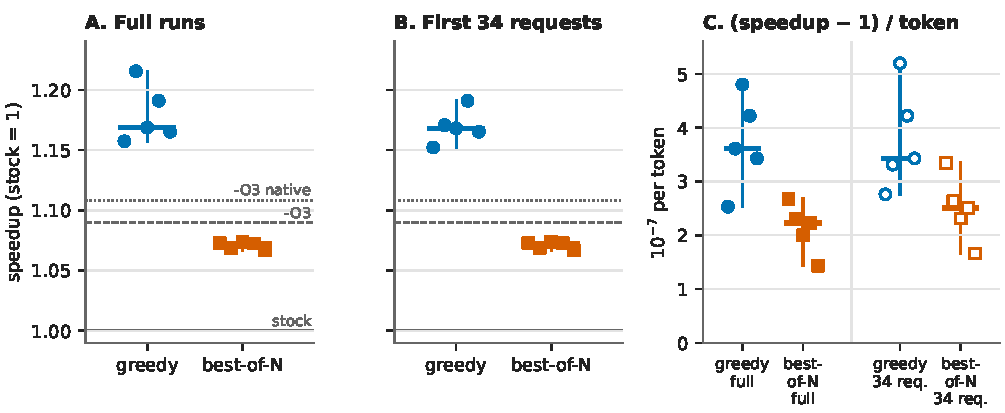
\includegraphics[width=\textwidth]{main_figure.pdf}
\caption{Per-seed results (one marker per seed; left to right = seeds 1--5), median (thick bar) and full range. A: full runs as executed. B: post hoc, best patch within the first 34 requests. C: metric B on both bases (filled: full; open: first 34 requests). All plotted values passed the frozen rule in 3/3 re-measurements. Dashed/dotted lines: C1 controls (separate batch and node).}
\label{fig:main}
\end{figure}
\textbf{Speedup.} Median (range) over five seeds, full runs: greedy 1.169 (1.157--1.216), best-of-N 1.073 (1.067--1.074); first 34 requests (post hoc): greedy 1.168 (1.152--1.191), best-of-N 1.073 (1.067--1.074). Greedy was higher in 5 of 5 paired seeds in both analyses. Exploratory exact two-sided tests (chosen after the data were seen, nothing was pre-specified): permutation test of the difference of medians p = 0.048 (both analyses), Mann--Whitney \cite{mann1947} p = 0.008 (full) and 0.008 (34 requests), sign test p = 0.0625. With five seeds per arm these p-values are coarse (the smallest possible Mann--Whitney p is 0.008).

\textbf{Tokens.} Full runs count all tokens of every request sent; the 34-request analysis counts the first 34 requests' cumulative tokens. Truncated replies (13 requests, 432,991 tokens) are counted. 10 requests returned HTTP 502 without a usage object: their consumption is unknown and not included, so token totals (4,233,676 over all runs) may underestimate cost and overstate efficiency. The course quotient is (best\_confirmed\_speedup $-$ 1)/total\_tokens from the last row of \texttt{credits.csv}; our rank-mode \texttt{credits.csv} has no confirmed column and \texttt{summary.json} keeps an unused default (1.0), so metric A is computed from \texttt{results.jsonl}: the best speedup among candidates whose two measurements both passed the frozen rule (it equals the search's best ranked value in all 10 runs, which is not itself used as the confirmed value). Metric B uses the independent re-measurement; they differ by under 2\% and the logs are unchanged. Median metric A, full runs: greedy 3.60 vs best-of-N 2.22 $\times$10$^{-7}$ (greedy higher in 4/5 seeds; permutation p = 0.048, Mann--Whitney p = 0.016); first 34 requests: 3.46 vs 2.49. Metric B agrees; all exploratory.

\textbf{Controls.} C1 (compiler), C2 (human) and the inert patch are five repeated measurements each on node xcnd24, from a different batch than the DeepSeek runs (Table~\ref{tab:ctl}). The -O3 gain (speedup $-$ 1) is 53\% of the greedy median gain; -O3 -march=native adds only 1.014 over -O3, below the 2\% gate (0/5 accepted). C3 is the best-of-N arm and C4 the five seeds per arm.

\textbf{C2 (human-directed, AI-assisted).} Attempt 1 replaces the linear scan in \texttt{Profile::GetMesg} by a 65,536-entry table built once by a function-local static object; attempt 2 adds a table for \texttt{Profile::GetFieldIndex} (message type $\times$ 256 field numbers, built on first call). Both are likely faster because these lookups run for every message and field of the decode. They were made by the author with AI assistance (Claude Code); no per-line authorship is recorded. The README asks for a timed hour before looking at any search output. \textbf{There is no stopwatch or timer record.} File modification times in the C2 directory span 10:20--11:11 on 2 November (51 minutes); the earliest search results file in \path{runs/} is 22:44 on 3 November. This is consistent with, but does not verify, a timed hour before any search output; \textbf{the author-reported time is not available to us and is not stated.}

\begin{table}[t]
\centering
\small
\setlength{\tabcolsep}{3.5pt}
\begin{tabular}{lrrr}
\toprule
Control (vs stock -O2 unless stated) & Speedup, median of 5 & Range & Accepted \\
\midrule
C1 -O3 & 1.090 & 1.088--1.092 & 5/5 \\
C1 -O3 -march=native & 1.108 & 1.106--1.108 & 5/5 \\
C1 -O3 -march=native vs -O3 & 1.014 & 1.014--1.016 & 0/5 \\
C2 human patch, attempt 1 & 1.068 & 1.067--1.069 & 5/5 \\
C2 human patch, attempt 2 & 1.082 & 1.082--1.082 & 5/5 \\
\bottomrule
\end{tabular}
\caption{Non-LLM references; five repeated measurements each (not independent seeds), node xcnd24. Source: \path{runs/phase1-final/controls.csv}.}
\label{tab:ctl}
\end{table}
\textbf{What the search patches are.} All five best-of-N winners rewrite \texttt{Profile::GetMesg} (a table lookup, the idea of human attempt 1); their speedups (1.067--1.074) are close to attempt 1 (1.068). \texttt{Profile::GetMesg} and \texttt{FieldBase::FieldBase} (copy constructor with member-initialiser list) were accepted in every greedy chain (7 to 12 accepted steps each). The submitted patch series is the median-seed greedy chain (seed 3), explained patch by patch in \path{patches/}; the other chains are experiment records, and each run's final patch has a short description in \path{experiments/patches/final-cumulative/README.md}. In the seed-3 chain four steps gave most of the search-time gain (\texttt{GetMesg} 6.1\%, \texttt{FieldBase} copy 4.4\%, \texttt{GetFieldIndex} 1.5\%, \texttt{AddField} 1.4\%) and six were below 0.3\%; none was independently confirmed.

\section{Limitations and conclusion}
\textbf{Budget and analysis.} Unequal budgets and the post hoc 34-request analysis are described in Section 3. All 10 runs and all failures are kept (13 truncated requests are in the token counts, 10 HTTP-502 requests have unknown token use and are not; compile, correctness and crash failures are in each \texttt{results.jsonl}).

\textbf{Measurement.} Calibration used a synthetic, stationary workload on one node with min-time about 0.06 s; the SDK was measured with 0.25 s on two node families, so the calibrated detection rates (reliable near a 5\% change, partial at 2\%) transfer only loosely. Ratios reduce, but do not remove, node differences: the same CPU model string gives about 359 ms on xcnc and 480 ms on xcnd, and we did not test whether a patch's effect depends on the node. CPU model recorded after the runs (all formal nodes Xeon E5-2620 v3, xcnc2 from the Phase 0 log).

\textbf{Correctness.} We ran only the harness checks of Section 2.3. Lookup tables built lazily behind a plain \texttt{bool} appear in four of the five best-of-N winners (seeds 1, 3, 4, 5; seed 2 initialises through a function-local static, which C++11 makes thread-safe), and the seed-3 greedy chain also caches the last queried message in mutable statics in \texttt{GetFieldIndex}; concurrent callers could race on this unsynchronised shared state. The human patches use function-local static objects and do not. \texttt{FieldBase::GetValue} in that chain assumes a little-endian host. Nothing was tested beyond single-threaded benchmark inputs; no patch is claimed ready for upstream.

\textbf{Conclusion.} \emph{Observed:} greedy chains reached a higher final speedup than best-of-N in all five seeds (median 1.169 vs 1.073), with higher token cost per run but a higher median speedup per token; best-of-N never exceeded -O3, and only greedy exceeded -O3 -march=native. \emph{Not established:} that greedy is better at equal resources in general; that the gap comes from selection, feedback or inheritance (the arms differ in start point, memory and token use; no ablation was run); or that the patches are correct beyond the checks listed.

\textbf{AI assistance.} Code, scripts, this report and patch commit messages were prepared with Claude Code (Anthropic) under the author's direction, who remains responsible for the claims. The patches of the automated search were generated by deepseek-v4.1-flash; the C2 patches are human-directed and AI-assisted. Build and run commands, file index and open items: \texttt{DELIVERY.md}.

\bibliographystyle{plain}
\bibliography{references}
\end{document}
